%\documentclass[hyperref={pdfpagelabels=false},slidetop,9pt]{beamer}
\documentclass[slidetop,8pt]{beamer}
\usepackage[T1]{fontenc}
\usepackage[utf8]{inputenc}
\newcommand{\nom}{Porte conteneur}
\newcommand{\sequence}{03}
\newcommand{\num}{04}
\newcommand{\type}{TD}
\newcommand{\descrip}{Résolution d'un problème en utilisant des méthodes algorithmiques}
\newcommand{\competences}{Alt-C3: Concevoir un algorithme répondant à un problème précisément posé}
\usepackage{etex}
\usepackage{tikz}
\usepackage[european]{circuitikz}
\usepackage{pgf}
\usepackage[all]{xy}
\usepackage{pgfpages}
\usepackage{graphbox}
\usepackage{pdfpages}
\usepackage[adobe-utopia]{mathdesign}
\usepackage{ifthen}
\usepackage{cancel}
\usepackage{framed}
\usepackage{subfig}
\usepackage{tabularx}
\usepackage{setspace}
\usepackage{soul}
\usepackage{schemabloc}
\usepackage{eqnarray}
\usepackage[dot, phantomtext]{dashundergaps}
\usepackage{media9}
\usepackage{multimedia}

\author{Renaud Costadoat}
\institute{Lycée Dorian}

\usepackage{multido}
\usepackage{multirow}
\usepackage{multicol} % Portions de texte en colonnes
\usepackage{flafter}%floatants après la référence

\usepackage{color}
\usepackage{xcolor}
\usepackage{colortbl}

\usepackage[gen]{eurosym}
\usepackage{tikz}
%\usepackage{pstricks,pst-node,pst-tree,pst-solides3d}
\usepackage{lmodern}
\usepackage[francais]{babel}
\usepackage{pslatex}
\usetheme{renaud}
\usepackage{times}
\usepackage{amsmath}
\usepackage{verbatim}
\usepackage{moreverb}
%\usetikzlibrary{arrows,shapes}
\usepackage{graphicx}
\usepackage{psfrag}
\usepackage{wrapfig}
\usepackage{etoolbox}

\definecolor{gris25}{gray}{0.75}
\definecolor{bleu}{RGB}{18,33,98}
\definecolor{bleuf}{RGB}{42,94,171}
\definecolor{bleuc}{RGB}{231,239,247}
\definecolor{rougef}{RGB}{185,18,27}
\definecolor{rougec}{RGB}{255,188,204}%255,230,231
\definecolor{vertf}{RGB}{103,126,82}
\definecolor{vertc}{RGB}{220,255,191}

\setlength\parindent{24pt}
\parskip 7.2pt
\parindent 8pt

\newenvironment{rem}[1][\hsize]%
{%
    \def\FrameCommand
   {%
\rotatebox{90}{\textit{\textsf{Remarque}}} 
       {\color{bleuf}\vrule width 3pt}%
       \hspace{0pt}%must no space.
       \fboxsep=\FrameSep\colorbox{bleuc}%
  }%
    \MakeFramed{\hsize#1\advance\hsize-\width\FrameRestore}%
}%
{\endMakeFramed}%


\newenvironment{savoir}[1][\hsize]%
{%
    \def\FrameCommand
    {%
\rotatebox{90}{\textit{\textsf{Savoir}}} 
        {\color{bleuf}\vrule width 3pt}%
        \hspace{0pt}%must no space.
        \fboxsep=\FrameSep\colorbox{bleuc}%
    }%
    \MakeFramed{\hsize#1\advance\hsize-\width\FrameRestore}%
}%
{\endMakeFramed}%

\newenvironment{prob}[1][\hsize]%
{%
    \def\FrameCommand%
    {%
\rotatebox{90}{\textit{\textsf{Problématique}}} 
        {\color{rougef}\vrule width 3pt}%
        \hspace{0pt}%must no space.
        \fboxsep=\FrameSep\colorbox{rougec}%
    }%
    \MakeFramed{\hsize#1\advance\hsize-\width\FrameRestore}%
}%
{\endMakeFramed}%

\newenvironment{obj}[1][\hsize]%
{%
    \def\FrameCommand%
    {%
\rotatebox{90}{\textit{\textsf{Objectif}}} 
        {\color{vertf}\vrule width 3pt}%
        \hspace{0pt}%must no space.
        \fboxsep=\FrameSep\colorbox{vertc}%
    }%
    \MakeFramed{\hsize#1\advance\hsize-\width\FrameRestore}%
}%
{\endMakeFramed}%

\newenvironment{defi}[1][\hsize]%
{%
    \def\FrameCommand%
    {%
\rotatebox{90}{\textit{\textsf{Definition}}} 
        {\color{bleuf}\vrule width 3pt}%
        \hspace{0pt}%must no space.
        \fboxsep=\FrameSep\colorbox{rougec}%
    }%
    \MakeFramed{\hsize#1\advance\hsize-\width\FrameRestore}%
}%
{\endMakeFramed}%


\newenvironment{hypo}[1][\hsize]%
{%
    \def\FrameCommand%
    {%
\rotatebox{90}{\textit{\textsf{Hypothèse\\}}} 
        {\color{bleuf}\vrule width 3pt}%
        \hspace{0pt}%must no space.
        \fboxsep=\FrameSep\colorbox{bleuc}%
    }%
    \MakeFramed{\hsize#1\advance\hsize-\width\FrameRestore}%
}%
{\endMakeFramed}%


\newenvironment{prop}[1][\hsize]%
{%
    \def\FrameCommand%
    {%
\rotatebox{90}{\textit{\textsf{Propriété}}} 
        {\color{bleuf}\vrule width 3pt}%
        \hspace{0pt}%must no space.
        \fboxsep=\FrameSep\colorbox{bleuc}%
    }%
    \MakeFramed{\hsize#1\advance\hsize-\width\FrameRestore}%
}%
{\endMakeFramed}%

\newenvironment{props}[1][\hsize]%
{%
    \def\FrameCommand%
    {%
\rotatebox{90}{\textit{\textsf{Propriétés}}} 
        {\color{bleuf}\vrule width 3pt}%
        \hspace{0pt}%must no space.
        \fboxsep=\FrameSep\colorbox{bleuc}%
    }%
    \MakeFramed{\hsize#1\advance\hsize-\width\FrameRestore}%
}%
{\endMakeFramed}%

\newenvironment{exemple}[1][\hsize]%
{%
    \def\FrameCommand%
    {%
\rotatebox{90}{\textit{\textsf{Exemple}}} 
        {\color{vertf}\vrule width 3pt}%
        \hspace{0pt}%must no space.
        \fboxsep=\FrameSep\colorbox{vertc}%
    }%
    \MakeFramed{\hsize#1\advance\hsize-\width\FrameRestore}%
}%
{\endMakeFramed}%

\newenvironment{resultat}[1][\hsize]%
{%
    \def\FrameCommand%
    {%
\rotatebox{90}{\textit{\textsf{Resultat}}} 
        {\color{rougef}\vrule width 3pt}%
%        {\color{bleuf}\vrule width 3pt}%
        \hspace{0pt}%must no space.
        \fboxsep=\FrameSep\colorbox{rougec}%
    }%
    \MakeFramed{\hsize#1\advance\hsize-\width\FrameRestore}%
}%
{\endMakeFramed}%

\newenvironment{methode}[1][\hsize]%
{%
    \def\FrameCommand%
    {%
\rotatebox{90}{\textit{\textsf{Méthode\\}}} 
        {\color{rougef}\vrule width 3pt}%
        \hspace{0pt}%must no space.
        \fboxsep=\FrameSep\colorbox{rougec}%
    }%
    \MakeFramed{\hsize#1\advance\hsize-\width\FrameRestore}%
}%
{\endMakeFramed}%

\newenvironment{theo}[1][\hsize]%
{%
    \def\FrameCommand%
    {%
\rotatebox{90}{\textit{\textsf{Théorème\\}}} 
        {\color{rougef}\vrule width 3pt}%
        \hspace{0pt}%must no space.
        \fboxsep=\FrameSep\colorbox{rougec}%
    }%
    \MakeFramed{\hsize#1\advance\hsize-\width\FrameRestore}%
}%
{\endMakeFramed}%

\newenvironment{warn}[1][\hsize]%
{%
    \def\FrameCommand%
    {%
\rotatebox{90}{\textit{\textsf{Attention\\}}} 
        {\color{rougef}\vrule width 3pt}%
        \hspace{0pt}%must no space.
        \fboxsep=\FrameSep\colorbox{rougec}%
    }%
    \MakeFramed{\hsize#1\advance\hsize-\width\FrameRestore}%
}%
{\endMakeFramed}%

% \usepackage{pstricks}
%\usepackage{minitoc}
% \setcounter{minitocdepth}{4}

\setcounter{tocdepth}{2}

% \mtcselectlanguage{french} 

%\usepackage{draftcopy}% "Brouillon"
% \usepackage{floatflt}
\usepackage{psfrag}
%\usepackage{listings} % Permet d'insérer du code de programmation
\renewcommand{\baselinestretch}{1.2}

% Changer la numérotation des figures :
% ------------------------------------
% \makeatletter
% \renewcommand{\thefigure}{\ifnum \c@section>\z@ \thesection.\fi
%  \@arabic\c@figure}
% \@addtoreset{figure}{section}
% \makeatother
 


%%%%%%%%%%%%
% Définition des vecteurs %
%%%%%%%%%%%%
 \newcommand{\vect}[1]{\overrightarrow{#1}}

%%%%%%%%%%%%
% Définition des torseusr %
%%%%%%%%%%%%

 \newcommand{\torseur}[1]{%
\left\{{#1}\right\}
}

\newcommand{\torseurcin}[3]{%
\left\{\mathcal{#1} \left(#2/#3 \right) \right\}
}

\newcommand{\torseurstat}[3]{%
\left\{\mathcal{#1} \left(#2\rightarrow #3 \right) \right\}
}

 \newcommand{\torseurc}[8]{%
%\left\{#1 \right\}=
\left\{
{#1}
\right\}
 = 
\left\{%
\begin{array}{cc}%
{#2} & {#5}\\%
{#3} & {#6}\\%
{#4} & {#7}\\%
\end{array}%
\right\}_{#8}%
}

 \newcommand{\torseurcol}[7]{
\left\{%
\begin{array}{cc}%
{#1} & {#4}\\%
{#2} & {#5}\\%
{#3} & {#6}\\%
\end{array}%
\right\}_{#7}%
}

 \newcommand{\torseurl}[3]{%
%\left\{\mathcal{#1}\right\}_{#2}=%
\left\{%
\begin{array}{l}%
{#1} \\%
{#2} %
\end{array}%
\right\}_{#3}%
}

 \newcommand{\vectv}[3]{%
\vect{V\left( {#1} \in {#2}/{#3}\right)}
}


\newcommand{\vectf}[2]{%
\vect{R\left( {#1} \rightarrow {#2}\right)}
}

\newcommand{\vectm}[3]{%
\vect{\mathcal{M}\left( {#1}, {#2} \rightarrow {#3}\right)}
}


 \newcommand{\vectg}[3]{%
\vect{\Gamma \left( {#1} \in {#2}/{#3}\right)}
}

 \newcommand{\vecto}[2]{%
\vect{\Omega\left( {#1}/{#2}\right)}
}

\newcommand{\reponse}[1][4]
{
\multido{}{#1}
{
\begin{center}
\makebox[0.9\linewidth]{\dotfill} \end{center}
}}


% }$$\left\{\mathcal{#1} \right\}_{#2} =%
% \left\{%
% \begin{array}{c}%
%  #3 \\%
%  #4 %
% \end{array}%
% \right\}_{#5}}


%  ------------------------------------------
% | Modification du formatage des sections : | 
%  ------------------------------------------

% Grands titres :
% ---------------

\newcommand{\titre}[1]{%
\begin{center}
      \bigskip
      \rule{\textwidth}{1pt}
      \par\vspace{0.1cm}
      
      \textbf{\large #1}
      \par\rule{\textwidth}{1pt}
    \end{center}
    \bigskip
  }

% Supprime le numéro du chapitre dans la numérotation des sections:
% -----------------------------------------------------------------
\makeatletter
\renewcommand{\thesection}{\@arabic\c@section}
\makeatother


% \titleformat{\chapter}[display]
% {\normalfont\Large\filcenter}
% {}
% {1pc}
% {\titlerule[1pt]
%   \vspace{1pc}%
%   \Huge}[\vspace{1ex}%
% \titlerule]


%%%% Chapitres Comme PY Pechard %%%%%%%%%
% numéro du chapitre
\DeclareFixedFont{\chapnumfont}{OT1}{phv}{b}{n}{80pt}
% pour le mot « Chapitre »
\DeclareFixedFont{\chapchapfont}{OT1}{phv}{m}{it}{40pt}
% pour le titre
\DeclareFixedFont{\chaptitfont}{T1}{phv}{b}{n}{25pt}

\definecolor{gris}{gray}{0.75}
\setbeamertemplate{section in toc}[sections numbered]

\newlength{\RoundedBoxWidth}
\newsavebox{\GrayRoundedBox}
\newenvironment{GrayBox}[1][\dimexpr\textwidth-4.5ex]%
   {\setlength{\RoundedBoxWidth}{\dimexpr#1}
    \begin{lrbox}{\GrayRoundedBox}
       \begin{minipage}{\RoundedBoxWidth}}%
   {   \end{minipage}
    \end{lrbox}
    \begin{center}
    \begin{tikzpicture}%
       \draw node[draw=bleuf,fill=bleuc,rounded corners,%
             inner sep=2ex,text width=\RoundedBoxWidth]%
             {\usebox{\GrayRoundedBox}};
    \end{tikzpicture}
    \end{center}}
    
\ifdef{\prive}{\pgfpagesuselayout{2 on 1}[a4paper,border shrink=0mm]}
\ifdef{\prive}{\setbeamertemplate{navigation symbols}{}}
\setbeamertemplate{itemize item}[ball]
%\setbeamertemplate{blocks}[rounded]%[shadow=true]
\setbeamercolor{block title}{fg=white,bg=grisf}        % titre block normal 
\setbeamercolor{block body}{fg=grisf,bg=grisc!50}      % corps block normal
\setbeamercolor{block body alerted}{fg=white,bg=warning}   % idem pour un block alerte

\title{\nom}
\date{S\sequence \ - \type\num}

\begin{document}
\shorthandoff{:!}
\bibliographystyle{abbrvnat-fr}

\usebackgroundtemplate%
{%
    \centering
\includegraphics[width=\paperwidth]{../../img/fond2}%
}

{
\setbeamertemplate{navigation symbols}{}
\setbeamertemplate{headline}[pagetitre]
\setbeamertemplate{footline}[pagetitre]
\usebackgroundtemplate{\centering
\includegraphics[width=\paperwidth]{../../img/fond}}
\frame{\titlepage}
}



\section{Introduction} 

\begin{frame}[fragile]
\frametitle{Introduction}

La bibliothèque NumPy (http://www.numpy.org/) permet d'effectuer des calculs numériques avec Python. Elle introduit une gestion facilitée des tableaux de nombres.

Il faut au départ importer le package numpy avec l'instruction suivante :

\begin{GrayBox}[0.85\textwidth]
\begin{verbatimtab}[3]
>>> import numpy as np
\end{verbatimtab}
\end{GrayBox}

Certaines variables sont prédéfinies comme la variable $\pi$.

\begin{GrayBox}[0.85\textwidth]
\begin{verbatimtab}[3]
>>> np.pi
3.141592653589793
\end{verbatimtab}
\end{GrayBox}

\end{frame}


\section{Tableaux et matrices} 

\begin{frame}[fragile]
\frametitle{Tableaux et matrices}

Le premier point fondamental de Numpy (et de Scipy) est la gestion des tableaux et des matrices grâce à la fonction objet \verb? array()?.

\begin{GrayBox}[0.85\textwidth]
\begin{verbatimtab}[3]
>>> np.array([1,2,3,4,5,6])
array([1, 2, 3, 4, 5, 6])
>>> np.array([1,2,3,4,5,6],'d')
array([ 1.,  2.,  3.,  4.,  5.,  6.])
>>> np.array([1,2,3,4,5,6],'D')
array([ 1.+0.j,  2.+0.j,  3.+0.j,  4.+0.j,  5.+0.j,  6.+0.j])
\end{verbatimtab}
\end{GrayBox}

Pour créer une matrice, vous pouvez utiliser \verb? array()? avec des listes de listes Python.

\begin{GrayBox}[0.85\textwidth]
\begin{verbatimtab}[3]
>>> np.array([[0,1],[1,0]],'d')
array([[ 0.,  1.],
       [ 1.,  0.]])
\end{verbatimtab}
\end{GrayBox}
\end{frame}

\begin{frame}[fragile]
\frametitle{Tableaux et matrices}

Vous pouvez aussi générer des matrices vides (remplies de zéros) de tailles arbitraires.

\begin{GrayBox}[0.85\textwidth]
\begin{verbatimtab}[3]
np.zeros((3,3),'d')
array([[ 0.,  0.,  0.],
       [ 0.,  0.,  0.],
       [ 0.,  0.,  0.]])
\end{verbatimtab}
\end{GrayBox}

Ainsi que des matrices identité avec la fonction \verb? identity()?.

\begin{GrayBox}[0.85\textwidth]
\begin{verbatimtab}[3]
>>> np.identity(4,'d')
array([[ 1.,  0.,  0.,  0.],
       [ 0.,  1.,  0.,  0.],
       [ 0.,  0.,  1.,  0.],
       [ 0.,  0.,  0.,  1.]])
\end{verbatimtab}
\end{GrayBox}
\end{frame}

\begin{frame}[fragile]
\frametitle{Opérations sur les matrices}

Les objets matrice font ce qu'il faut lorsqu'ils sont multipliés par des scalaires :

\begin{GrayBox}[0.85\textwidth]
\begin{verbatimtab}[3]
>>> 0.125*np.identity(3,'d')
array([[ 0.125,  0.   ,  0.   ],
       [ 0.   ,  0.125,  0.   ],
       [ 0.   ,  0.   ,  0.125]])
\end{verbatimtab}
\end{GrayBox}

Addition de deux matrices (sous réserve toutefois qu'elles soient de mêmes dimensions).

\begin{GrayBox}[0.85\textwidth]
\begin{verbatimtab}[3]
>>> np.identity(2,'d') + np.array([[1,1],[1,2]])
array([[ 2.,  1.],
       [ 1.,  3.]])
\end{verbatimtab}
\end{GrayBox}

\end{frame}

\begin{frame}[fragile]
\frametitle{Opérations sur les matrices}

Multiplication de matrice et produit scalaire.

\begin{GrayBox}[0.85\textwidth]
\begin{verbatimtab}[3]
>>> np.dot(np.identity(2),np.ones((2,2)))
array([[ 1.,  1.],
       [ 1.,  1.]])
>>> v = np.array([3,4],'d')
>>> np.sqrt(np.dot(v,v))
5.0
\end{verbatimtab}
\end{GrayBox}

Produit vectoriel.

\begin{GrayBox}[0.85\textwidth]
\begin{verbatimtab}[3]
>>> u = np.array([1,2,3])
>>> v = np.array([4,5,6])
>>> np.cross(u,v)	
array([-3,  6, -3])
\end{verbatimtab}
\end{GrayBox}

\end{frame}

\begin{frame}[fragile]
\frametitle{Opérations sur les matrices}

Multiplication de matrices membres à membres

\begin{GrayBox}[0.85\textwidth]
\begin{verbatimtab}[3]
>>> a=np.array([1,2,3])
>>> b=np.array([3,2,1])
>>> np.multiply(a,b)
array([3, 4, 3])
\end{verbatimtab}
\end{GrayBox}

\end{frame}

\begin{frame}[fragile]
\frametitle{Opérations sur les matrices}

La fonction \verb? shape ? permet de déterminer la dimension d'une matrice.

\begin{GrayBox}[0.85\textwidth]
\begin{verbatimtab}[3]
>>> m = np.array([[1,2],[3,4]])
>>> m.shape
(2,2)
\end{verbatimtab}
\end{GrayBox}

Les fonctions \verb? determinant() ?, \verb? inverse() ? et \verb? transpose() ? produisent les résultats attendus. Une transposition peut être abrégée en plaçant \verb? .T ? à la fin d'un nom d'objet matrice.

\begin{GrayBox}[0.85\textwidth]
\begin{verbatimtab}[3]
>>> m = np.array([[1,2],[3,4]])
>>> m.T
array([[1, 3],
       [2, 4]])
\end{verbatimtab}
\end{GrayBox}

\end{frame}

\section{Espace linéaire, fonctions matricielles et tracés} 

\begin{frame}[fragile]
\frametitle{Espace linéaire, fonctions matricielles et tracés}

La fonction objet \verb? linspace(start, end, nb)? crée un tableau espace linéaire de points de valeurs comprises entre \verb? start (inclus)? et \verb? end (inclus)? en un nombre \verb? nb ? de points.

\begin{GrayBox}[0.95\textwidth]
\begin{verbatimtab}[3]
>>> np.linspace(0,1,20)
array([ 0.        ,  0.05263158,  0.10526316,  0.15789474,  0.21052632,
        0.26315789,  0.31578947,  0.36842105,  0.42105263,  0.47368421,
        0.52631579,  0.57894737,  0.63157895,  0.68421053,  0.73684211,
        0.78947368,  0.84210526,  0.89473684,  0.94736842,  1.        ])
\end{verbatimtab}
\end{GrayBox}

\begin{minipage}{0.45\linewidth}
\begin{GrayBox}[0.85\textwidth]
Cette fonction permet de tracer des données pour un graphique.\\
\begin{verbatimtab}[3]
x = np.linspace(0,2*np.pi)
plt.plot(x,np.cos(x))
\end{verbatimtab}
\end{GrayBox}
\end{minipage}\hfill
\begin{minipage}{0.45\linewidth}
 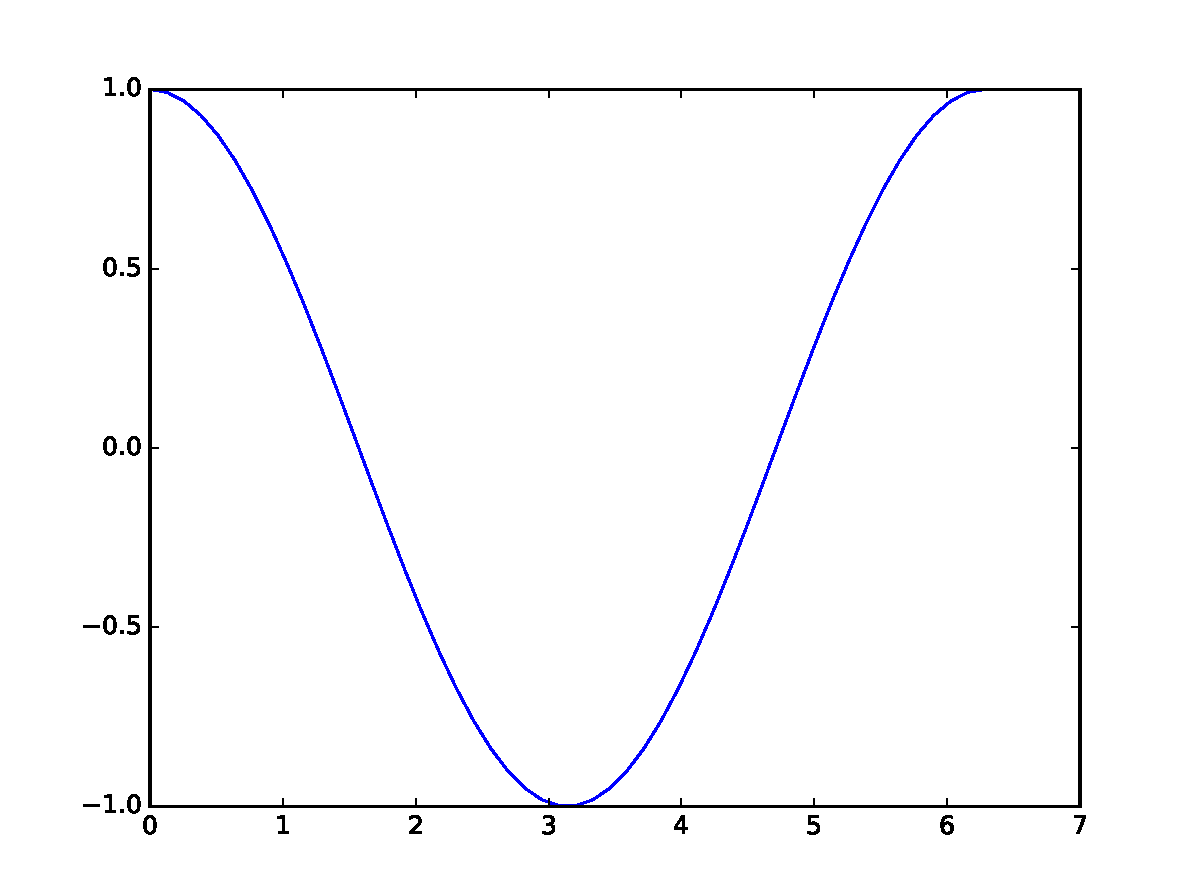
\includegraphics[width=0.8\linewidth]{img/figure_1}
\end{minipage}

\end{frame}

\begin{frame}[fragile]
\frametitle{Espace linéaire: Exercice}
Proposer le code permettant de tracer la figure suivante présentant, pour un solide en translation:\\
\begin{minipage}{0.46\linewidth}
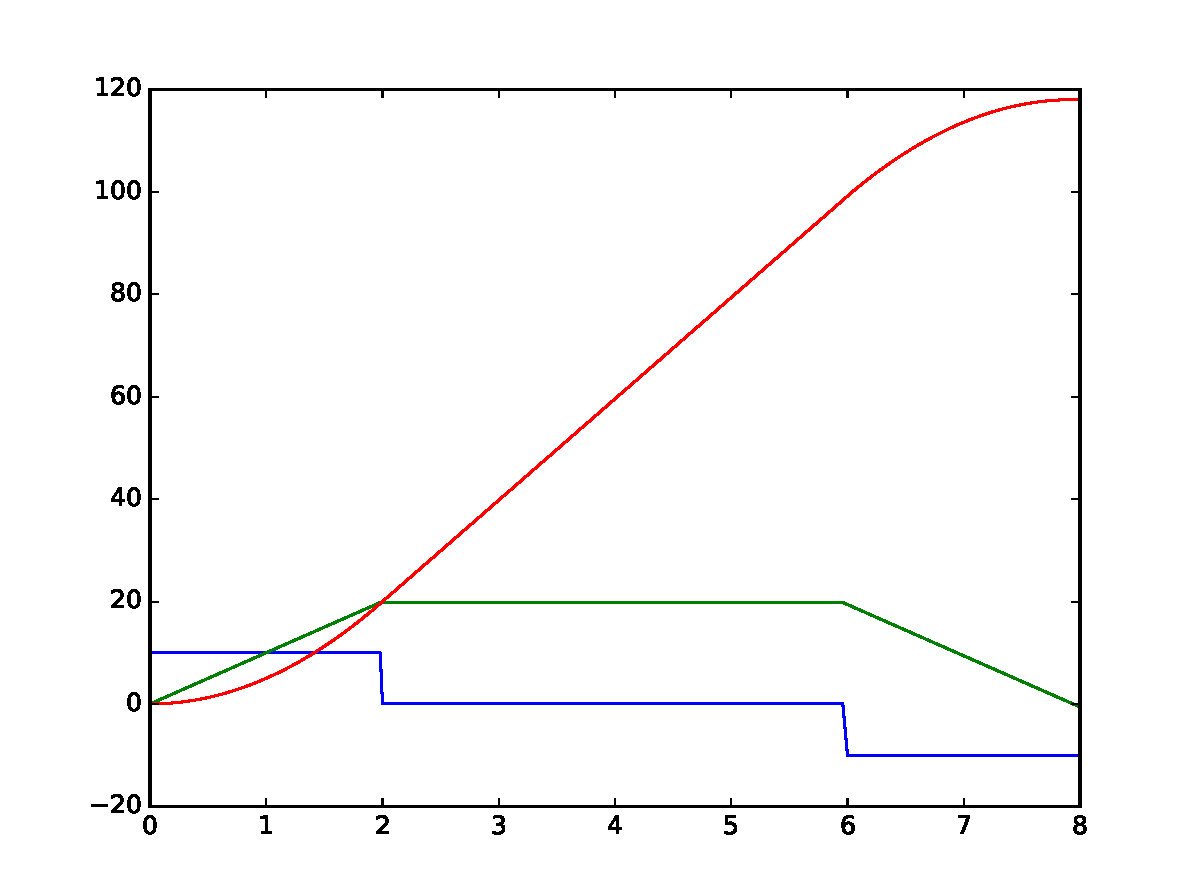
\includegraphics[width=0.8\linewidth]{img/figure_2}
\end{minipage}\hfill
\begin{minipage}{0.46\linewidth}
\begin{itemize}
 \item l'accélération (en bleu),
 \item la vitesse (en vert),
 \item la position (en rouge).
\end{itemize}
\end{minipage}
\vspace{3cm}
\end{frame}

\section{Solveurs matriciels}

\begin{frame}[fragile]
\frametitle{Solveurs matriciels}

Il est possible de résoudre des systèmes d'équations linéaires avec la fonction \verb? solve() ?.

\begin{center}
$\left\{\begin{array}{l}
x+y+z=6 \\ 2*y+5*z=-4 \\ 2*x+5*y-z=27
\end{array}\right.$
\end{center}

\begin{GrayBox}[0.85\textwidth]
\begin{verbatimtab}[3]
>>> A = np.array([[1,1,1],[0,2,5],[2,5,-1]])
>>> b = np.array([6,-4,27])
>>> np.linalg.solve(A,b)
array([ 5.,  3., -2.])
\end{verbatimtab}
\end{GrayBox}

\end{frame}

\begin{frame}[fragile]
\frametitle{Solveurs matriciels}
Plusieurs fonctions pour calculer des valeurs propres ainsi que des vecteurs propres :

\begin{itemize}
 \item \verb? eigvals()? retourne les valeurs propres d'une matrice
 \item \verb? eigvalsh()? retourne les valeurs propres d'une matrice hermitienne,
 \item \verb? eig()? retourne les valeurs propres et les vecteurs propres d'une matrice,
 \item \verb? eigh()? retourne les valeurs propres et les vecteurs propres d'une matrice hermitienne.
\end{itemize}

\begin{GrayBox}[0.85\textwidth]
\begin{verbatimtab}[3]
>>> A = np.array([[13,-4],[-4,7]],'d')
>>> np.linalg.eigvalsh(A)
array([  5.,  15.])
>>> np.linalg.eigh(A)
(np.array([  5.,  15.]), np.array([[-0.4472136 , -0.89442719],
        [-0.89442719,  0.4472136 ]]))
\end{verbatimtab}
\end{GrayBox}
\end{frame}


\begin{frame}[fragile]
\frametitle{Solveurs matriciels: Exercice}
Proposer un code utilisant la bibliothèque Numpy permettant de résoudre le système d'équations suivant.

\begin{flushleft}
$\left\{\begin{array}{l}
x-3*y+8*z=-16 \\ 2*x+3*y-4*z=24 \\ 2*y-3*z=7 \\ 8*x-3*z=17
\end{array}\right.$
\end{flushleft}
\vspace{3cm}
\end{frame}

\end{document}
